% Please use the skeleton file you have received in the
% invitation-to-submit email, where your data are already
% filled in. Otherwise please make sure you insert your
% data according to the instructions in PoSauthmanual.pdf
\documentclass{PoS}

\usepackage{amsmath}
\usepackage{xspace}   % decides whether to insert a space or not
\usepackage{fixmath}
\usepackage{bm,braket}
\usepackage[mathcal]{euscript}
\usepackage{wrapfig}

% Definitions
\newcommand{\calB}{\mathcal B}
\newcommand{\calS}{\mathcal S}
\newcommand{\calH}{\mathcal H}
\newcommand{\order}[1]{{{\cal O}\left(#1\right)}}
\newcommand{\ttbar}{\ensuremath{t \bar t}\xspace}
\newcommand{\qqbar}{\ensuremath{q \bar q}\xspace}
\newcommand{\qbar}{\ensuremath{\bar q}\xspace}
\newcommand{\bfw}{\bm{w}}
\newcommand{\gammaE}{\gamma_E}
\newcommand{\ie}{{\it i.e. }}

\title{Top pair production at NNLO: an alternative approach}

\ShortTitle{Top pair production at NNLO: an alternative approach}

\author{\speaker{Sebastian Sapeta}\thanks{
  Based on work done in collaboration with Micha\l{} Czakon and Ren\'e
  \'Angeles-Mart\'inez.
  }\\
  %
  Institute of Nuclear Physics, Polish Academy of Sciences \\
  ul.\ Radzikowskiego 152, 31-342 Krak\'ow, Poland\\
  %
  E-mail: \email{sebastian.sapeta@ifj.edu.pl}}

\abstract{
We report on progress towards developing a framework for calculation of the NNLO
cross section for top quark pair production. Our approach combines the
$q_T$-slicing method and small-$q_T$ factorization, and its main technical
challenge comes down to evaluation of the soft function at NNLO. We develop a
framework based on sector decomposition and present a proof-of-concept
calculation of the $n_f$ part of the NNLO soft function.
}

\FullConference{13th International Symposium on Radiative Corrections\\
		24-29 September, 2017\\
		St. Gilgen, Austria}

\begin{document}

%-----------------------------------------------------------------------------
\section{Introduction}

The increasing precision of the LHC data sets very high demands on the accuracy
of theoretical predictions. The latter involve, in particular, corrections from
higher perturbative orders of Quantum Chromodynamics.
%
In this regard, the state of the art for most processes of interest has very
recently changed from NLO to NNLO. Some gaps still need to be filled, however,
and additional work is required to fully test the NNLO results and implement
them in efficient public codes such that they can benefit experimental analyses.
%
At the same time, the seminal calculation of the N$^3$LO cross section for the
Higgs boson production from gluon fusion~\cite{Anastasiou:2015ema} has marked
the first step on the way towards pushing the accuracy of QCD predictions to the
next level.

One of the most important processes measured at the LHC is the production of the
top quark pair.  It is relevant both in studies of properties of the Standard
Model, as well as in searches for new physics, as it forms significant
backgrounds to many signatures. The cross section for this process is currently
known up to NNLO~\cite{Baernreuther:2012ws, Czakon:2012pz, Czakon:2012zr, Czakon:2013goa, Czakon:2015owf, Czakon:2016ckf}.

In this proceedings, we present a proof-of-concept calculation of the $n_f$ part
of the NNLO soft function for top quark pair production. This result, together
with the framework and tools developed to obtain it, form key  elements of
an alternative calculation of the complete NNLO cross section for that process.

The motivation behind our work is two-fold. On one hand, it will lead to a
second, independent result for the NNLO top pair production cross section,
which, given the complexity of the calculation, is highly desirable.
At the same time, our work forms a stepping stone towards developing a general
framework for calculations of N$^3$LO QCD corrections to a wide range of
processes of relevance for hadron colliders.


%-----------------------------------------------------------------------------
\section{Theoretical framework}

The approach for achieving NNLO accuracy for the top pair production,
presented in this proceedings, is part of a wider strategy for calculating
N$^m$LO contributions to processes of the type
%
\begin{equation}
  h_1 + h_2 \to F\, {\textstyle (q_T)} + X\,,
  %\label{eq:}
\end{equation}
%
where two hadrons, $h_1$ and $h_2$, collide and produce an object $F$, which is
registered in a detector, together with an undetected QCD radiation $X$. 
%
Our framework is suitable both when $F$, whose transverse momentum is denoted by
$q_T$, is a colour-neutral object (single EW boson, pair of EW bosons, the
Higgs) as well as when it carries colour, like in the case of the top quark
pair. 

We use the $q_T$-slicing method, which allows us to write the cross as a sum of
two components, each of which is separately finite~\cite{Catani:2007vq,
Bonciani:2015sha}
%
\begin{equation}
  \frac{\sigma_{{\rm N}^m{\rm LO}}^{F}}{d\Phi} = 
  %\sigma_{{\rm N}^m{\rm LO}}^{F} = 
  \int^{q_{T{\rm cut}}}_0 
  \!\!\!\!\! d q_T\,
  \frac{d\sigma^{F}_{{\rm N}^m{\rm LO}}}{d\Phi dq_T} +
  \int_{q_{T{\rm cut}}}^\infty 
  \!\!\!\!\! d q_T\,
  \frac{d\sigma^{F + {\rm jet}}_{{\rm N}^{m-1}{\rm LO}}}{d\Phi dq_T}\,.
  \label{eq:qT-slicing}
\end{equation}
%
The advantage of this approach is that the second term in
Eq.~(\ref{eq:qT-slicing}), which represents resolved emissions, is required only
at the N$^{m-1}$LO accuracy, and, in most interesting cases, it is already
known.  On the contrary, the first term, which combines virtual and unresolved
real corrections, is usually unknown. However it is needed only in the
small-$q_T$ approximation.

In order to calculate the latter we use the Soft Collinear Effective
Theory~(SCET)~\cite{Becher:2014oda}, in which the cross section factorizes at
small $q_T$ according to the formula
%
\begin{equation}
  \frac{d\sigma^F_{{\rm N}^m{\rm LO}}}{d\Phi dq_T} = 
  \calB_1^{{\rm N}^m{\rm LO}}\otimes
  \calB_2^{{\rm N}^m{\rm LO}}\otimes
  \calH^{{\rm N}^m{\rm LO}}\otimes
  \calS^{{\rm N}^m{\rm LO}} +
  \order{\frac{q_T^2}{q^2}} \,,
  \label{eq:smallqT-cs}
\end{equation}
%
where $q^2$ is an invariant mass of the object $F$.
%
The functions appearing in the above equation account for contributions from
different phase space regions of $X$. Specifically, the beam functions $\calB_i$
sum up emissions of collinear and anti-collinear partons, the hard functions,
$\calH$, accounts for hard radiation, and the soft function, $\calS$, sums
emissions from soft, real gluons.
%
Calculation of each of these functions is significantly simpler than 
calculation of the complete cross section. In addition, some of the functions
are already available from literature.

In the case of the top quark pair production, the beam functions are known up to
NNLO~\cite{Gehrmann:2012ze,Gehrmann:2014yya} and the NNLO hard function can be
extracted from Refs.~\cite{Czakon:2008zk, Baernreuther:2013caa}. However, the
small-$q_T$ soft function is only known up to NLO~\cite{Li:2013mia,
Catani:2014qha}. Hence, in order to achieve the NNLO accuracy of the \ttbar
cross section, one needs to calculate the missing NNLO correction to the soft
function appearing in Eq.~(\ref{eq:smallqT-cs}) (We note that such calculation
shares many features with that of the NNLO soft function for boosted tops in the
threshold limit~\cite{Ferroglia:2012uy}. However, the result for the latter is
not of direct use in our context.)

The soft function for our process of interest can be schematically defined with
the following equation
%
\begin{equation}
  {\textstyle S(q_T,\beta,\theta) } = \sum 
  \!\!\!\! \!\!
  \vcenter{\hbox{
  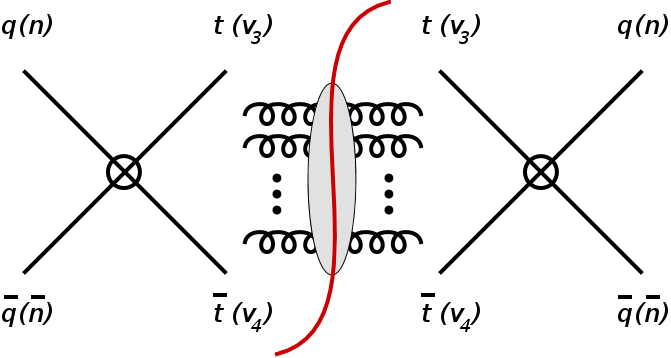
\includegraphics[width=0.39\textwidth]{plots/sf-schematic.png}}}
  {\textstyle \delta\left(q_T - \left|\sum_i k_{i\perp} \right|\right)
  \prod_i \delta^{+}(k_i^2) }\,.
  \label{eq:sf-all-orders}
\end{equation}
%
To this end, we focus on the $\qqbar \to \ttbar$ subprocess and introduce the
following notation for the 4-momenta: 
$p_q = m_t n$, $p_{\bar q} = m_t \bar n$ and 
$p_t = m_t v_3 + l_3$, $p_{\bar t} = m_t v_4 + l_4$, where 
$n = (1,0,0,1)$, $\bar n = (1,0,0,-1)$. 
%The N$^m$LO soft function
%%of Eq.~(\ref{eq:sf-all-orders}) is construted by 
%is constructed by attaching $m$ soft gluons to the external partons in all
%possible ways.  Eq.~(\ref{eq:sf-all-orders}) corresponds to a sum of such
%contributions to all orders. 
%
We see that in the definition~(\ref{eq:sf-all-orders}), the transverse
momenta of real emissions are restricted to sum up to a fixed value of $q_T$.
Because the gluons are soft, $l_i \ll m_t v_i$, and the velocities satisfy Born
kinematics, $n+\bar n = v_3 + v_4$, at each perturbative order. Apart from
$q_T$, the soft function of Eq.~(\ref{eq:sf-all-orders}) depends on $\beta =
\sqrt{1-4m_t^2/q^2}$ and $\theta$, where the latter is the scattering angle of
the top quark in the \ttbar rest frame.

The NNLO soft function corresponds to a sum of all $\order{\alpha_s^2}$
contributions from Eq.~(\ref{eq:sf-all-orders}). They take forms of
$2d$-dimensional integrals which exhibit soft and rapidity singularities. The
latter arise when the light-cone components of gluons 4-momenta become very
small or very large, and are not removed by dimensional regularization. In our
calculation, we adopt the prescription of Ref.~\cite{Becher:2011dz} which turns
the above divergences into poles in a new regulator $\alpha$. Even though the
individual integrals suffer from rapidity divergences, their complete sum, hence
the soft function, is finite in the limit $\alpha \to 0$~\cite{Li:2013mia,
Becher:2011dz}.

To calculate the soft function at this order, we designed the following
integration strategy that can be algorithmically applied to evaluate each of its
contributions. We start from analytically integrating 3 out of $2d$ dimensions.
Then, we map the remaining momenta into a unit hypercube (splitting the integral
if necessary) and apply sector decomposition~\cite{Binoth:2000ps,Binoth:2003ak}
to disentangle overlapping singularities. Finally, we expand the result in
$\alpha$ and $\epsilon$ and numerically integrate the coefficients with help of
the CUBA library~\cite{Hahn:2004fe}.


%-----------------------------------------------------------------------------
%\section{Results}
\section{Proof of concept}

In order to validate our framework, we calculated the complete $n_f$
contribution to the NNLO soft function, which involves diagrams from
Eq.~(\ref{eq:sf-all-orders}) with one gluon on each side of the cut and the blob
replaced with the quark loop. 

The $n_f$ contribution has the advantage that it can be also obtained
analytically. Integration over the quark loop momentum proceeds in a similar
manner to the standard calculation of the vacuum polarization, only that now the
tensor structure involves also the vector $n$, which is a consequence of
introducing the rapidity regulator discussed above. One is then left with the
integral over gluon momentum which we performed with help of the method of
differential equations. 
%
The $n_f$ part of the NNLO soft function can be also singled out from the prediction of the Renormalization Group allowing for an additional cross check.

As mentioned in the previous section, all $\alpha$ poles have to cancel in the
complete soft function. They also need to cancel within the subset of diagrams
contributing to the $n_f$ part. And indeed, our analytic result contains
contributions like
%
\begin{equation}
  \bfw_{13}^{q\qbar} I_{13} + \bfw_{24}^{q\qbar} I_{24}   =
  \bfw_{13}^{q\qbar} \left(
  -\frac{8}{3\epsilon\alpha} +\frac{8}{3\epsilon\alpha}
  -\frac{8(5+3\gammaE+2\ln2)}{9\alpha}
  +\frac{8(5+3\gammaE+2\ln2)}{9\alpha}
  + \ldots
  \right)\,,
  %\label{eq:}
\end{equation}
%
while from the numeric, sector decomposition-based approach, we obtain
%
\begin{equation}
  \bfw_{13}^{q\qbar} I_{13} + \bfw_{24}^{q\qbar} I_{24}   =
  \bfw_{13}^{q\qbar} \left(
  -\frac{2.66597}{\epsilon\alpha} +\frac{2.66597}{\epsilon\alpha}
  -\frac{4.13986}{\alpha}
  +\frac{4.13986}{\alpha}
  + \ldots
  \right)\,.  
  %\label{eq:}
\end{equation}
%
In the above equations, $\bfw_{ij}$ and $I_{ij}$ correspond, respectively, to
the colour matrix and the phase space integral parts of graphs in which the soft
gluons are attached to the external lines $i$ and $j$, where we identify
$(1,2,3,4) \leftrightarrow (n,\bar n, v_3, v_4)$.

As a second step of our validation, we checked that the result for the $n_f$
part of the NNLO soft function obtained through direct calculation with the
strategy described in the preceding section reproduces exactly all terms
predicted by the Renormalization Group (see \cite{Li:2013mia, Ferroglia:2012uy}
for details), \ie terms proportional to $\displaystyle \frac{1}{\epsilon^2}$,
$\displaystyle \frac{1}{\epsilon}$, $\ln^2\mu$ and $\ln\mu$.

\begin{figure}[t]
 \begin{center}
 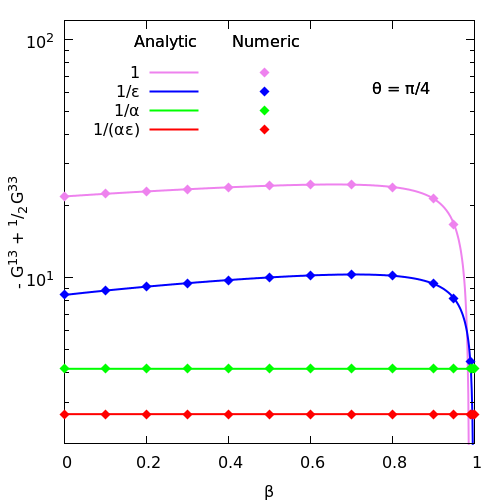
\includegraphics[width=0.45\textwidth]{../../vp-terms/plots/bubble-beta13.png}
 \hfill
 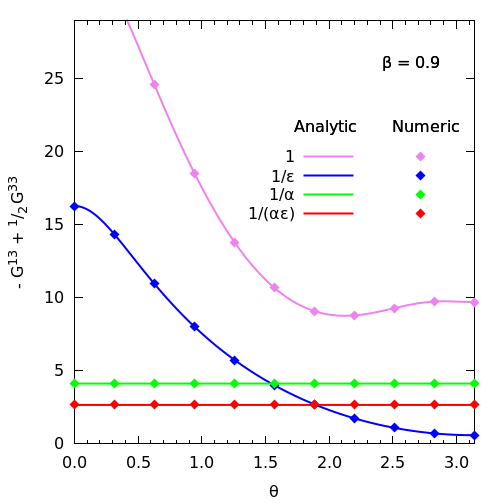
\includegraphics[width=0.45\textwidth]{../../vp-terms/plots/bubble-theta13.png}
 \end{center}
 \caption{
 Comparison of numeric and analytic results for example graphs contributing to
 the $n_f$ part of the NNLO soft function. See text for details.
 }
 \label{fig:compG13}
\end{figure}


As a final step in the proof of concept of our approach to calculation of the
NNLO soft function for top pair production, we compared numerical results for
combinations of quark-bubble graphs, obtained with the sector
decomposition-based method, and the analytic results from the method of
differential equations. An example comparison is presented in
Fig.~\ref{fig:compG13} (see Ref.~\cite{ReneMttD} for another example) where
points (lines) correspond to numeric (analytic) coefficients of different powers
in the expansion in $\alpha$ and $\epsilon$. We observe per-mille-level
agreement for this and all the remaining graphs that contribute to the $n_f$
part of the NNLO soft function.

%-----------------------------------------------------------------------------
\section{Conclusions}

We presented a proof-of-concept calculation of the $\alpha_s^2 n_f$
contribution to the small-$q_T$ soft function for top quark pair production. In
order to evaluate the necessary divergent integrals we developed a framework
based on sector decomposition. 
%
We performed a three-step validation of our results: by verifying that
rapidity singularities cancel, by cross-checking that our direct calculation
reproduces all terms predicted by the Renormalization Group and, finally, by
finding a perfect agreement between numeric results from the sector
decomposition-based framework and analytic results for individual graphs.
%
The concepts and tools developed in our study allow for evaluation of all
remaining integrals needed for calculation of the NNLO soft function and are
generalizable to higher orders. Together with the $q_T$-slicing method, they
offer  a approach for calculation of the top quark pair production cross
section at NNLO.

%-----------------------------------------------------------------------------
\section*{Acknowledgements}

This work has been supported by the National Science Centre, Poland grant
POLONEZ  
\begin{wrapfigure}[4]{r}{0.15\textwidth}
  \centering
  \vspace{-10pt}
  
\includegraphics[width=0.15\textwidth]{plots/flag_yellow_low.jpg}
\end{wrapfigure}
%
No. 2015/19/P/ST2/03007. 
%
The project has received funding from the
European Union's Horizon 2020 research  and  innovation  programme  under  the
Marie Sk\l{}odowska-Curie grant agreement No. 665778.
%
We are grateful to Mateusz Dobija for implementation of numerical integration
with CUBA.  

%\clearpage

\begin{thebibliography}{99}

%\cite{Anastasiou:2015ema}
\bibitem{Anastasiou:2015ema}
  C.~Anastasiou, C.~Duhr, F.~Dulat, F.~Herzog and B.~Mistlberger,
  %``Higgs Boson Gluon-Fusion Production in QCD at Three Loops,''
  Phys.\ Rev.\ Lett.\  {\bf 114} (2015) 212001
  doi:10.1103/PhysRevLett.114.212001
  [arXiv:1503.06056 [hep-ph]].
  %%CITATION = doi:10.1103/PhysRevLett.114.212001;%%

%\cite{Baernreuther:2012ws}
\bibitem{Baernreuther:2012ws}
  P.~B\"arnreuther, M.~Czakon and A.~Mitov,
  %``Percent Level Precision Physics at the Tevatron: First Genuine NNLO QCD
  %Corrections to $q \bar{q} \to t \bar{t} + X$,''
  Phys.\ Rev.\ Lett.\  {\bf 109} (2012) 132001
  doi:10.1103/PhysRevLett.109.132001
  [arXiv:1204.5201 [hep-ph]].
  %%CITATION = doi:10.1103/PhysRevLett.109.132001;%%

%\cite{Czakon:2012pz}
\bibitem{Czakon:2012pz}
  M.~Czakon and A.~Mitov,
  %``NNLO corrections to top pair production at hadron colliders: the
  %quark-gluon reaction,''
  JHEP {\bf 1301} (2013) 080
  doi:10.1007/JHEP01(2013)080
  [arXiv:1210.6832 [hep-ph]].
  %%CITATION = doi:10.1007/JHEP01(2013)080;%%

%\cite{Czakon:2012zr}
\bibitem{Czakon:2012zr}
  M.~Czakon and A.~Mitov,
  %``NNLO corrections to top-pair production at hadron colliders: the
  %all-fermionic scattering channels,''
  JHEP {\bf 1212} (2012) 054
  doi:10.1007/JHEP12(2012)054
  [arXiv:1207.0236 [hep-ph]].
  %%CITATION = doi:10.1007/JHEP12(2012)054;%%

%\cite{Czakon:2013goa}
\bibitem{Czakon:2013goa}
  M.~Czakon, P.~Fiedler and A.~Mitov,
  %``Total Top-Quark Pair-Production Cross Section at Hadron Colliders Through
  %$O(α\frac{4}{S})$,''
  Phys.\ Rev.\ Lett.\  {\bf 110} (2013) 252004
  doi:10.1103/PhysRevLett.110.252004
  [arXiv:1303.6254 [hep-ph]].
  %%CITATION = doi:10.1103/PhysRevLett.110.252004;%%

%\cite{Czakon:2015owf}
\bibitem{Czakon:2015owf}
  M.~Czakon, D.~Heymes and A.~Mitov,
  %``High-precision differential predictions for top-quark pairs at the LHC,''
  Phys.\ Rev.\ Lett.\  {\bf 116} (2016) no.8,  082003
  doi:10.1103/PhysRevLett.116.082003
  [arXiv:1511.00549 [hep-ph]].
  %%CITATION = doi:10.1103/PhysRevLett.116.082003;%%

%\cite{Czakon:2016ckf}
\bibitem{Czakon:2016ckf}
  M.~Czakon, P.~Fiedler, D.~Heymes and A.~Mitov,
  %``NNLO QCD predictions for fully-differential top-quark pair production at
  %the Tevatron,''
  JHEP {\bf 1605} (2016) 034
  doi:10.1007/JHEP05(2016)034
  [arXiv:1601.05375 [hep-ph]].
  %%CITATION = doi:10.1007/JHEP05(2016)034;%%

%\cite{Catani:2007vq}
\bibitem{Catani:2007vq}
  S.~Catani and M.~Grazzini,
  %``An NNLO subtraction formalism in hadron collisions and its application to
  %Higgs boson production at the LHC,''
  Phys.\ Rev.\ Lett.\  {\bf 98} (2007) 222002
  doi:10.1103/PhysRevLett.98.222002
  [hep-ph/0703012].
  %%CITATION = doi:10.1103/PhysRevLett.98.222002;%%

%\cite{Bonciani:2015sha}
\bibitem{Bonciani:2015sha}
  R.~Bonciani, S.~Catani, M.~Grazzini, H.~Sargsyan and A.~Torre,
  %``The $q_T$ subtraction method for top quark production at hadron
  %colliders,''
  Eur.\ Phys.\ J.\ C {\bf 75} (2015) no.12,  581
  doi:10.1140/epjc/s10052-015-3793-y
  [arXiv:1508.03585 [hep-ph]].
  %%CITATION = doi:10.1140/epjc/s10052-015-3793-y;%%

%\cite{Becher:2014oda}
\bibitem{Becher:2014oda}
  T.~Becher, A.~Broggio and A.~Ferroglia,
  %``Introduction to Soft-Collinear Effective Theory,''
  Lect.\ Notes Phys.\  {\bf 896} (2015) pp.1
  doi:10.1007/978-3-319-14848-9
  [arXiv:1410.1892 [hep-ph]].
  %%CITATION = doi:10.1007/978-3-319-14848-9;%%

%\cite{Gehrmann:2012ze}
\bibitem{Gehrmann:2012ze}
  T.~Gehrmann, T.~Lubbert and L.~L.~Yang,
  %``Transverse parton distribution functions at next-to-next-to-leading order:
  %the quark-to-quark case,''
  Phys.\ Rev.\ Lett.\  {\bf 109} (2012) 242003
  doi:10.1103/PhysRevLett.109.242003
  [arXiv:1209.0682 [hep-ph]].
  %%CITATION = doi:10.1103/PhysRevLett.109.242003;%%

%\cite{Gehrmann:2014yya}
\bibitem{Gehrmann:2014yya}
  T.~Gehrmann, T.~Luebbert and L.~L.~Yang,
  %``Calculation of the transverse parton distribution functions at
  %next-to-next-to-leading order,''
  JHEP {\bf 1406} (2014) 155
  doi:10.1007/JHEP06(2014)155
  [arXiv:1403.6451 [hep-ph]].
  %%CITATION = doi:10.1007/JHEP06(2014)155;%%

%\cite{Czakon:2008zk}
\bibitem{Czakon:2008zk}
  M.~Czakon,
  %``Tops from Light Quarks: Full Mass Dependence at Two-Loops in QCD,''
  Phys.\ Lett.\ B {\bf 664} (2008) 307
  doi:10.1016/j.physletb.2008.05.028
  [arXiv:0803.1400 [hep-ph]].
  %%CITATION = doi:10.1016/j.physletb.2008.05.028;%%

%\cite{Baernreuther:2013caa}
\bibitem{Baernreuther:2013caa}
  P.~B\"arnreuther, M.~Czakon and P.~Fiedler,
  %``Virtual amplitudes and threshold behaviour of hadronic top-quark
  %pair-production cross sections,''
  JHEP {\bf 1402} (2014) 078
  doi:10.1007/JHEP02(2014)078
  [arXiv:1312.6279 [hep-ph]].
  %%CITATION = doi:10.1007/JHEP02(2014)078;%%

%\cite{Li:2013mia}
\bibitem{Li:2013mia}
  H.~T.~Li, C.~S.~Li, D.~Y.~Shao, L.~L.~Yang and H.~X.~Zhu,
  %``Top quark pair production at small transverse momentum in hadronic
  %collisions,''
  Phys.\ Rev.\ D {\bf 88} (2013) 074004
  doi:10.1103/PhysRevD.88.074004
  [arXiv:1307.2464 [hep-ph]].
  %%CITATION = doi:10.1103/PhysRevD.88.074004;%%

%\cite{Catani:2014qha}
\bibitem{Catani:2014qha}
  S.~Catani, M.~Grazzini and A.~Torre,
  %``Transverse-momentum resummation for heavy-quark hadroproduction,''
  Nucl.\ Phys.\ B {\bf 890} (2014) 518
  doi:10.1016/j.nuclphysb.2014.11.019
  [arXiv:1408.4564 [hep-ph]].
  %%CITATION = doi:10.1016/j.nuclphysb.2014.11.019;%%

\bibitem{Ferroglia:2012uy}
  A.~Ferroglia, B.~D.~Pecjak, L.~L.~Yang, B.~D.~Pecjak and L.~L.~Yang,
  %``The NNLO soft function for the pair invariant mass distribution of boosted
  %top quarks,''
  JHEP {\bf 1210} (2012) 180
  doi:10.1007/JHEP10(2012)180
  [arXiv:1207.4798 [hep-ph]].
  %%CITATION = doi:10.1007/JHEP10(2012)180;%%

%\cite{Becher:2011dz}
\bibitem{Becher:2011dz}
  T.~Becher and G.~Bell,
  %``Analytic Regularization in Soft-Collinear Effective Theory,''
  Phys.\ Lett.\ B {\bf 713} (2012) 41
  doi:10.1016/j.physletb.2012.05.016
  [arXiv:1112.3907 [hep-ph]].
  %%CITATION = doi:10.1016/j.physletb.2012.05.016;%%

%\cite{Binoth:2000ps}
\bibitem{Binoth:2000ps}
  T.~Binoth and G.~Heinrich,
  %``An automatized algorithm to compute infrared divergent multiloop
  %integrals,''
  Nucl.\ Phys.\ B {\bf 585} (2000) 741
  doi:10.1016/S0550-3213(00)00429-6
  [hep-ph/0004013].
  %%CITATION = doi:10.1016/S0550-3213(00)00429-6;%%

\bibitem{Binoth:2003ak}
  T.~Binoth and G.~Heinrich,
  %``Numerical evaluation of multiloop integrals by sector decomposition,''
  Nucl.\ Phys.\ B {\bf 680} (2004) 375
  doi:10.1016/j.nuclphysb.2003.12.023
  [hep-ph/0305234].
  %%CITATION = doi:10.1016/j.nuclphysb.2003.12.023;%%

%\cite{Hahn:2004fe}
\bibitem{Hahn:2004fe}
  T.~Hahn,
  %``CUBA: A Library for multidimensional numerical integration,''
  Comput.\ Phys.\ Commun.\  {\bf 168} (2005) 78
  doi:10.1016/j.cpc.2005.01.010
  [hep-ph/0404043].
  %%CITATION = doi:10.1016/j.cpc.2005.01.010;%%

\bibitem{ReneMttD}
  R. Angeles-Martinez,
  {\it Proceedings of the XXXIX International Conference of Theoretical Physics
  ``Matter to the Deepest'' 2017, Podlesice, Poland}, 
  Acta Phys. Polon. B (2017).

\end{thebibliography}

\end{document}
